\subsection{Закон сохранения энергии и типы орбит}
Для движения тела c массой $m$ в гравитационном  в поле тела 
с массой \linebreak $M\gg m$ со скорость $v$ на расстоянии $r$ от 
гравитационного центра справедливо следующее соотношение: 
\begin{equation}
\frac{m v^2}{2}-\frac{GM m }{r}=E_0,
\end{equation}
где $E_0$ --- постоянная величина, если на тело не действуют
внешние силы кроме силы притяжения к центральному телу, 
равная сумме кинетической и потенциальной энергии тела. Данное равенство принято называть \term{законом сохранения энергии} для тела, движущегося в поле консервативных (потенциальных) сил.

\begin{wrapfigure}[11]{l}{.5\tw}
	\centering
	\vspace{-1.2pc}
	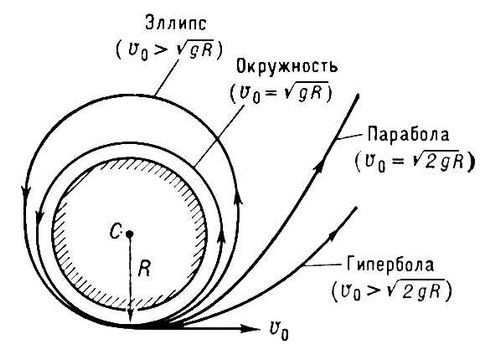
\includegraphics[width = 0.5\tw]{Space-speed}
	\caption{Возможные траектории тела \label{pic:orbits}}
\end{wrapfigure}
Если $E_0>0$, то траектория тела~--- \imp{гипербола}, 
ветви которой асимптотически приближаются к двум прямым. Стоит заметить,
что на бесконечно большом удалении тела с массой $m$ от массивного тела
его скорость остается положительной, так как суммарная энергия $E_0$ 
больше нуля.

Если $E_0=0$, то траектория тела~--- \imp{парабола}. При стремлении
расстояния $r$ между телами к бесконечности, скорость тела с стремится к нулю.

Отсюда становится очевидно, что на параболической и гиперболический
 траекториях движение тела не ограничено (инфинитно). 

Если $E_0<0$, то траектория тела~--- \imp{эллипс}. При 
эллиптической траектории движение ограничено (финитно), так как малое тело
не может бесконечно удалять с неотрицательной скоростью по причине того,
что суммарная энергия меньше нуля.

На Рис.\,\ref{pic:orbits} представлены примеры возможных траекторий тела 
относительно центрального (точка C). При $v_0 > v_{2}$ --- тело движется 
по гиперболе, при $v_0 = v_{2}$ --- по параболе, 
а при $v_0 < v_{2}$ --- по эллипсу.\\

\term{Первая космическая скорость} --- минимальная скорость, необходимая для 
того, чтобы маломассивное тело стало искусственным спутником центрального тела.
\begin{equation}v_1=\sqrt{\frac{GM}{R}}
\end{equation}
где $M$ --- масса массивного тела. Отсюда несложно получить выражение для
скорости искусственного небесного тела на высоте 
$h$.\begin{equation}v_h=\sqrt{\frac{GМ}{R+h}}=\sqrt{\frac{gR^2}{R+h}}
\end{equation}

\term{Параболическая} или \term{вторая космическая скорость} --- 
минимальная скорость, необходимая для того, чтобы маломассивное тело преодолело 
гравитационное притяжение центрального тела и покинуло замкнутую орбиту вокруг 
последнего. Выражение для которой имеет следующий вид:\begin{equation}
v_{2}=\sqrt{\frac{2GM}{r}}
\end{equation}

Для стабильной системы, частный случай~--- тело на круговой орбите, справедлива 
\term{теорема о вириале}:
\begin{equation}
2 \langle T\rangle 
= -\sum _{{k=1}}^{N}\langle {F}_{k}\cdot {r}_{k}\rangle 
= \langle U \rangle
\end{equation}

Где $\langle T\rangle$ --- средняя полная кинетическая энергия, $F_k$ --- сила, 
действующая на $k$-ю частицу. Другими словами, удвоенная средняя полная 
кинетическая энергия $T$ равна средней полной потенциальной энергии $U$. 

Применяя теорему о вириале для тела, обращающегося по круговой орбите можно 
получить выражения для первой космической скорость.
%\begin{table}[h!]
%\centering
%\begin{tabular}{|c|c|c|}
%\hline
%\textbf{Планета} & $\mathbf{v_1}$,~\textbf{км/c} & 
%$\mathbf{v_2}$,~\textbf{км/c}\\
%\hline
%Солнце & 436,8 & 617,7\\
%\hline
%Меркурий & 3,0 & 4,3\\
%\hline
%Венера & 7,4 & 10,5\\
%\hline
%Земля & 7,9 & 11,2\\
%\hline
%Луна & 1,7 & 2,4\\
%\hline
%Марс & 3,5 & 5,0\\
%\hline
%Юпитер & 42,0 & 59,5\\
%\hline
%Сатурн & 25,1 & 35,5\\
%\hline
%Уран & 15,0 & 21,3\\
%\hline
%Нептун & 16,6 & 23,5\\
%\hline
%\end{tabular}
%\caption{$v_1$ и $v_2$ на некоторых телах Солнечной системы}
%\end{table}




